\documentclass[slitetop]{beamer}
\mode<presentation>
{
  \setbeamertemplate{background canvas}[vertical shading][bottom=white!10,top=white!10]
  \usetheme{Warsaw}
}
% \usepackage{pgf,pgfarrows,pgfnodes,pgfautomata,pgfheaps,pgfshade}
\setbeamercovered{dynamic}
\usefonttheme[onlylarge]{structurebold}
\setbeamerfont*{frametitle}{size=\normalsize,series=\bfseries}
% \setbeamertemplate{navigation symbols}{}

% Standard packages
\usepackage{hyperref}
\usepackage[english]{babel}
\usepackage[utf8]{inputenc}
\usepackage[T1]{fontenc}
\usepackage{times}
\usepackage{amssymb}
\usepackage{textcomp}
\usepackage{color}

\title{Writing Scalable Network Applications in Python}
\subtitle{Prezentacja Pracy Dyplomowej}

\author{Łukasz Dobrzański\\ Promotor: dr inż. Andrzej Głowacz}
\institute{Katedra Telekomunikacji \\
Akademia Górniczo-Hutnicza im. Stanisława Staszica w Krakowie}

\date{16 Grudnia, 2009}

\begin{document}
\begin{frame}
  \titlepage
\end{frame}

\begin{frame}{Plan prezentacji}
  \tableofcontents
\end{frame}

\section{Wprowadzenie}
\subsection{Temat pracy}

\begin{frame}{Poruszane zagadnienia}
\begin{itemize}
\item{Skalowalność} 	%optymalizacja kodu pod wzgledem sklowalnosci
\item{Bezpieczeństwo} %podtawowe problemy aplikacji sieciowych
\item{Elastyczność rozwoju} % mozliwość elastycznych zmian na wielu plaszczyznach aplikacji
\end{itemize}
\end{frame}

\begin{frame}{Poruszane zagadnienia c.d.}
\begin{alertblock}{Wydajność}<+->
Definiuje  ilość czasu potrzebna do realizacji danej funkcji. Przykład: \textit{0.1 sek/rządanie}.
\end{alertblock}
\begin{alertblock}{Przepustowość}<+->
Definiuje maksymalną ilość informacji (zmian stanu)  jaka może być przetworzona przez system.\\ Przykład: \textit{120 kb/sek}.
\end{alertblock}
\begin{exampleblock}{Skalowalność}<+->
Określa zdolność systemu do pracy przy wzrastającym trendzie użytkowania lub ze zwieszającym się rozmiarem danych wejściowych.   
\end{exampleblock}
\end{frame}

\subsection{Motywacja}

\begin{frame}{Dlaczego ten projekt ?}
\begin{itemize}
\item{Skalowalność}
\item{Podobne applikacje}
\item{Osobiste zainteresowania}
\item{Perspektywy rozwoju projektu}
\end{itemize}
\end{frame}

\subsection{Użyte techonologie}

\begin{frame}{Główne komponenty}
\begin{itemize}
\item{Platforma Google App Engine}\uncover<2>{ \alert<2>{$40\%$} }
\item{Framework  Django}\uncover<2>{ \alert<2>{$30\%$} }
\item{System kontroli wersji Mercurial}\uncover<2>{ \alert<2>{$20\%$} }
\item{Środowisko Cocoa}\uncover<2>{ \alert<2>{$10\%$} }
\end{itemize}
\end{frame}

\section{Omówienie pracy}
\subsection{Opis projektu}

\begin{frame}{Architektura aplikacji}
\begin{figure}
	\begin{center}
		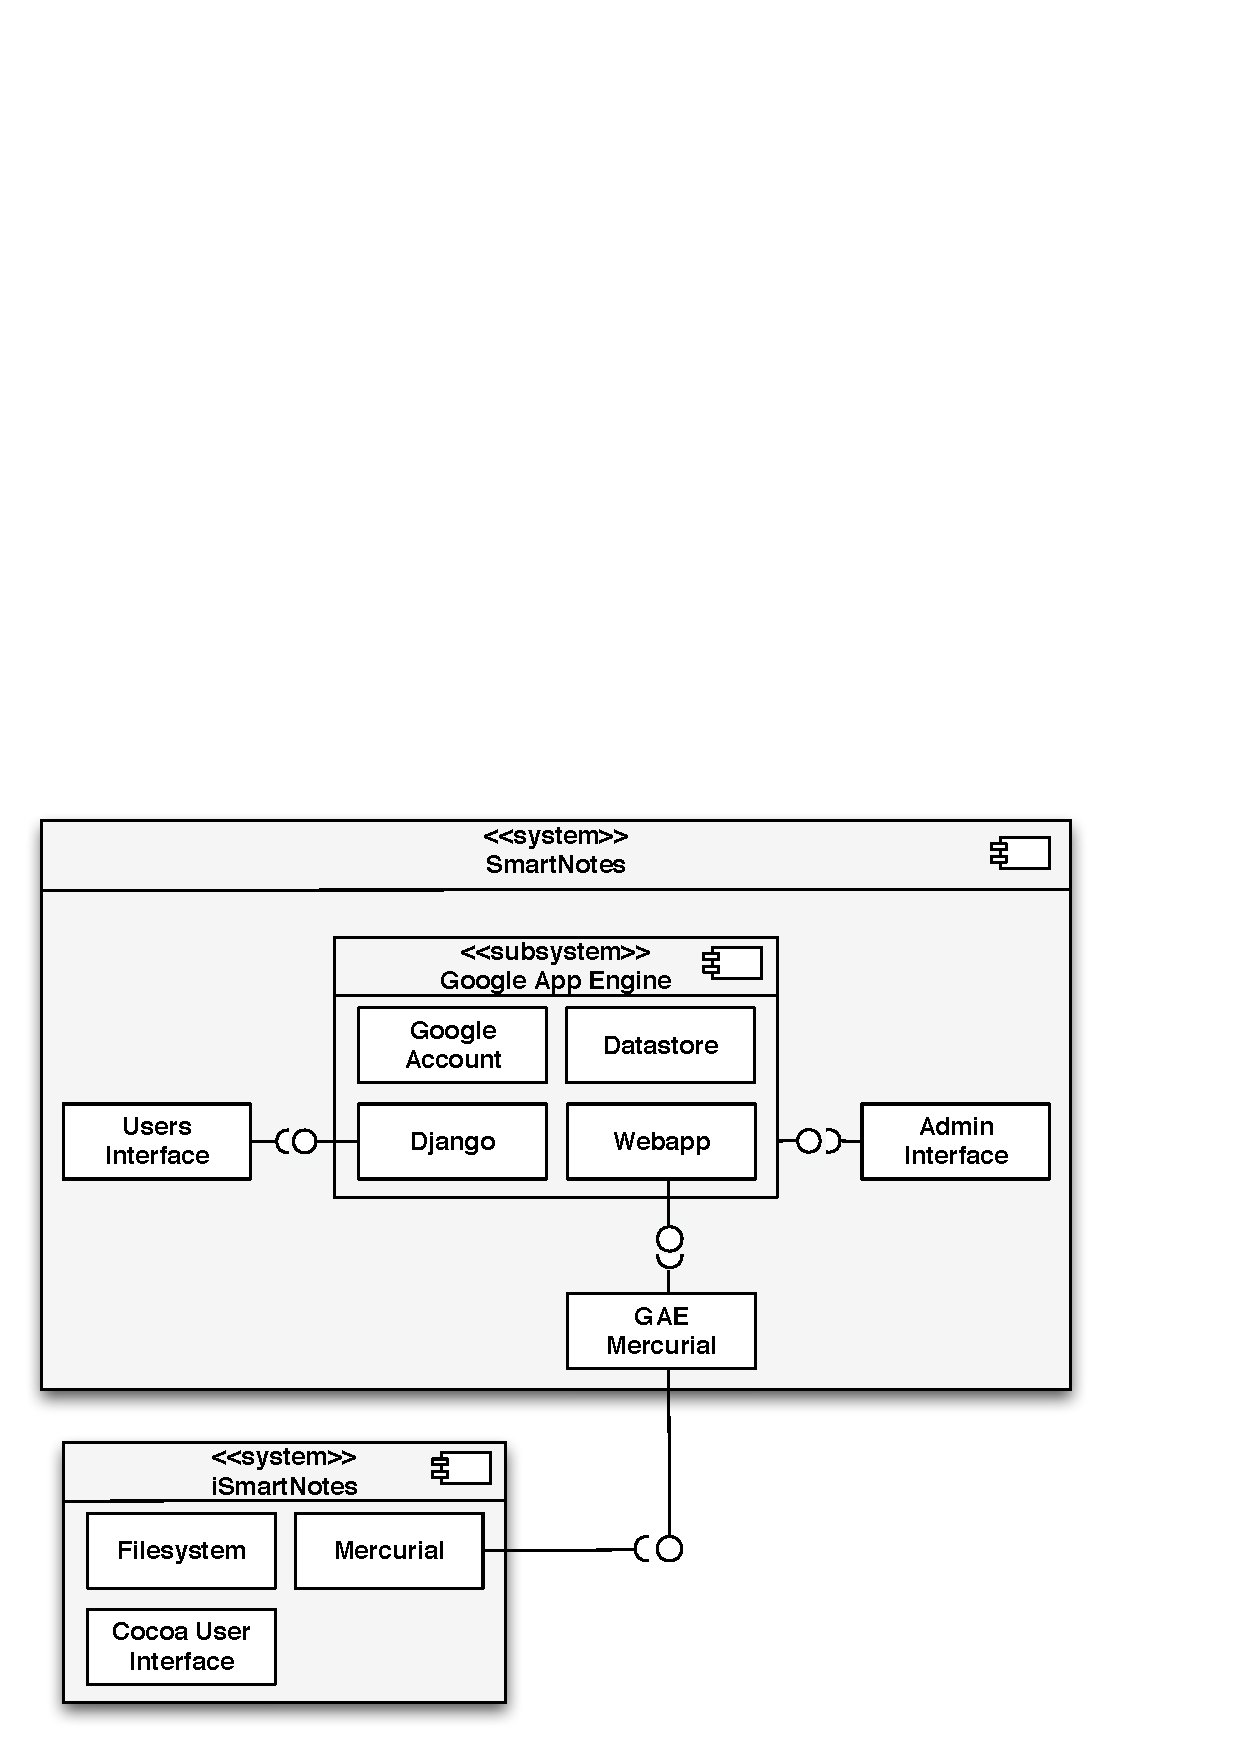
\includegraphics[scale=0.42]{../charts/smartnotes_componets.pdf}
  		\label{fig:smartnotes_components}
	\end{center}
\end{figure}
\end{frame}

\subsection{Ograniczenia i zalety}

\begin{frame}{Zestawienie}
\begin{columns}
  \column{.5\textwidth}
    \begin{alertblock}{Ograniczenia}<1-5,11>
    \begin{itemize}
        \item<1- | alert@+> Restrykcje ze strony GAE
        \item<2- | alert@+> Spojenie z  framewokiem
        \item<3- | alert@+> Poziom zależności od firmy Google
        \item<4- | alert@+> Współpraca środowisk GAE
        \item<5- | alert@+> Wsparcie dla REST
  \end{itemize}
  \end{alertblock}
  \column{.5\textwidth}
    \begin{exampleblock}{Zalety}<6-10,11>
    \begin{itemize}
        \item<6- | alert@+> Skalowalność
        \item<7- | alert@+> Niski koszt utrzymania 
        \item<8- | alert@+> Wysoka elastyczność w sferze wybranego środowiska 
        \item<9- | alert@+> Dostęp do najczęściej wykorzystywanych komponentów
        \item<10- | alert@+> Wygodny i wysoce użyteczny panel administracyjny
    \end{itemize}
    \end{exampleblock}
\end{columns}
\end{frame}



\section{Podsumowanie}
\subsection{Opracowane i sprawdzone rozwiązania}

\begin{frame}{}
\begin{itemize}
\item{Keszowanie}
\item{Dzielenie danych i skalowanie poziome}
\item{Minimalizowanie zbytecznego kodu}
\item{Wizja całości}
\end{itemize}
\end{frame}

\begin{frame}{}
\begin{center}
\huge{Dziękuję za uwagę}
\end{center}
\end{frame}

\end{document}